\documentclass[main.tex]{subfiles}
\begin{document}
\section{Telegrafenrauschen in Samarium-Erbium-Ferrit}

\subsection{Extraktion des Telegrafenrauschens}

\begin{figure}[h]
    \centering
    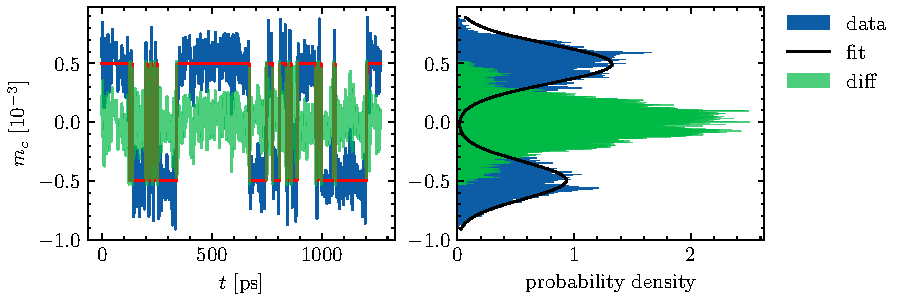
\includegraphics{bilder/plots/Bz_0mT/mc_fit_hist_part2_26.03meV.pdf}
    \caption{Extraktion aus \SI{1,2}{\nano\s}}\label{fig:Extraktion-ausschnitt}
\end{figure}
\todo{Bild ohne zuerst ohne diff?}
\todo{vergleich mit kmeans?}


\subsection*{Dominanz des Telegrafenrauschens}

\begin{figure}[h]
    \centering
    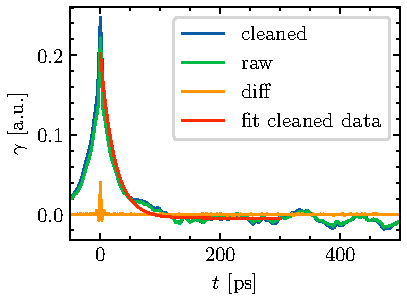
\includegraphics{bilder/plots/Bz_0mT/autocorr_26.03meV.pdf}
    \caption{vergleich Autokorrelation}\label{fig:autocorr}
\end{figure}

\subsection{Simulation ohne externes Magnetfeld}
\subsubsection{In der Zeitdomäne}
\begin{figure}[H]
    \centering
    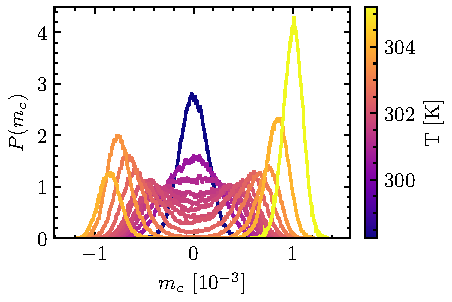
\includegraphics{bilder/plots/temp_comparison/mc_hist.pdf}
    \caption{temp hist}\label{fig:temp-hist}    
\end{figure}

\subsubsection{In der Frequenzdomäne}

\begin{figure}[H]
    \centering
    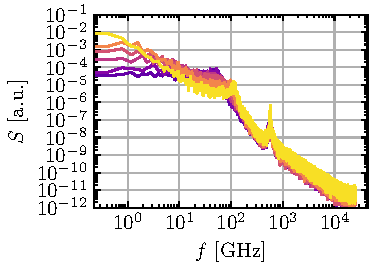
\includegraphics{bilder/plots/temp_comparison/spectral_power_density.pdf}
    \caption{temp fft}\label{fig:temp-fft}
\end{figure}


\subsection{Simulation mit externem Magnetfeld}
\subsubsection{In der Zeitdomäne}

\begin{figure}[H]
    \centering
    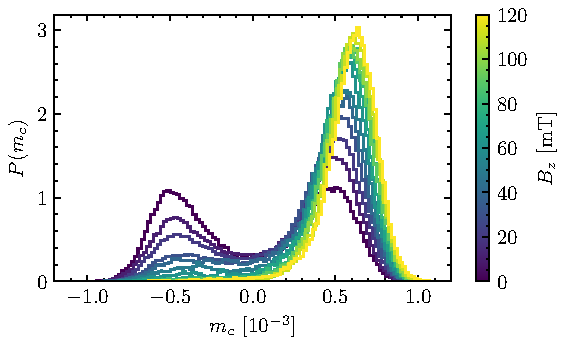
\includegraphics{bilder/plots/max_Bz/mc_hist.pdf}
    \caption{b hist}\label{fig:b-hist}    
\end{figure}

\subsubsection{In der Frequenzdomäne}


% bibliography (temporary)
% \bibliography{literatur} \todo{comment out before compiling main.tex}

\end{document}